\documentclass[11pt]{standalone}
\usepackage{amssymb}
\usepackage{amsmath}
\usepackage[no-math]{fontspec}
\usepackage{unicode-math}
\usepackage{libertinus}
\usepackage{pgf,xcolor}
\usepackage{tikz}
\usetikzlibrary{arrows.meta, backgrounds}
\usepackage{pgfplots}
\pgfplotsset{compat=newest}

\definecolor{my_darkgray}{HTML}{484949}
\definecolor{my_lightgray}{HTML}{F3F4F4}
\definecolor{my_darkblue}{HTML}{005A94}
\definecolor{my_lightblue}{HTML}{CCDEE9}
\definecolor{my_yellow}{HTML}{FFEC7F}
\definecolor{my_red}{HTML}{E60000}
\definecolor{my_orange}{HTML}{E87846}

\begin{document}
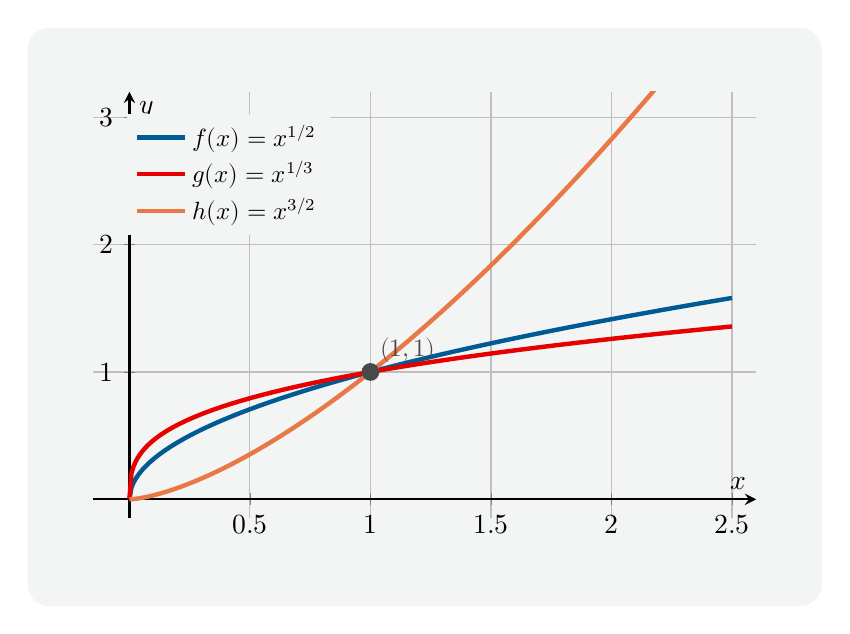
\begin{tikzpicture}[
    show background rectangle,
    background rectangle/.style={fill=my_lightgray, rounded corners=8pt},
    inner frame sep=0.8cm
]
\begin{axis}[
    axis lines=center,
    xlabel={$x$},
    ylabel={$y$},
    height=7cm, width=10cm,
    xmin=-0.15, xmax=2.6,
    ymin=-0.15, ymax=3.2,
    xtick={0, 0.5, 1, 1.5, 2, 2.5},
    ytick={0, 1, 2, 3},
    grid=both,
    axis line style={thick},
    legend style={
        font=\small,
        at={(0.05, 0.95)},
        anchor=north west,
        draw=none,
        fill=my_lightgray,
    },
    legend cell align=left,
]

% Three root functions, all with domain [0, inf).
% At x=0: all equal 0.  At x=1: all equal 1.
% For x in (0,1):  x^{1/3} > x^{1/2} > x^{3/2}
% For x > 1:       x^{3/2} > x^{1/2} > x^{1/3}
% The three curves visually "fan out" from (0,0) and (1,1).

% f(x) = x^{1/2} = sqrt(x)
\addplot[draw=my_darkblue, samples=300, ultra thick, domain=0:2.5]{x^0.5};
\addlegendentry{$f(x)=x^{1/2}$}

% g(x) = x^{1/3}  (grows slower than sqrt for x > 1)
\addplot[draw=my_red, samples=300, ultra thick, domain=0:2.5]{x^(1/3)};
\addlegendentry{$g(x)=x^{1/3}$}

% h(x) = x^{3/2}  (grows faster than sqrt for x > 1)
\addplot[draw=my_orange, samples=300, ultra thick, domain=0:2.5]{x^1.5};
\addlegendentry{$h(x)=x^{3/2}$}

% Mark the common point (1, 1) where all three curves intersect
\addplot[only marks, mark=*, mark size=3pt,
         draw=my_darkgray, fill=my_darkgray]
    coordinates{(1,1)};
\node[above right, font=\small, my_darkgray] at (axis cs:1,1) {$(1,1)$};

\end{axis}
\end{tikzpicture}
\end{document}
